%%-------------------------process on a circle---------------------------------------%%
\blue{
discuss about data generation on a circle, 
\begin{itemize}
\item including circulant matrix
\item why circulant matrix
\item discuss covarince, biasness and the difficulties of estimation
\item 
\end{itemize}
}
Using the covarince function $C_1e^{-a|\Delta\lambda|}$ and estimate empirical covarince from MOM as follows,

\beq\label{cov:circle1}
C(\theta) = \frac{1}{n_L} \sum_{i=1}^{n_L} (X(a_i+\theta)\cdot X(a_i))-(\overline{X(a)})^2
\eeq

\begin{figure}
\centering
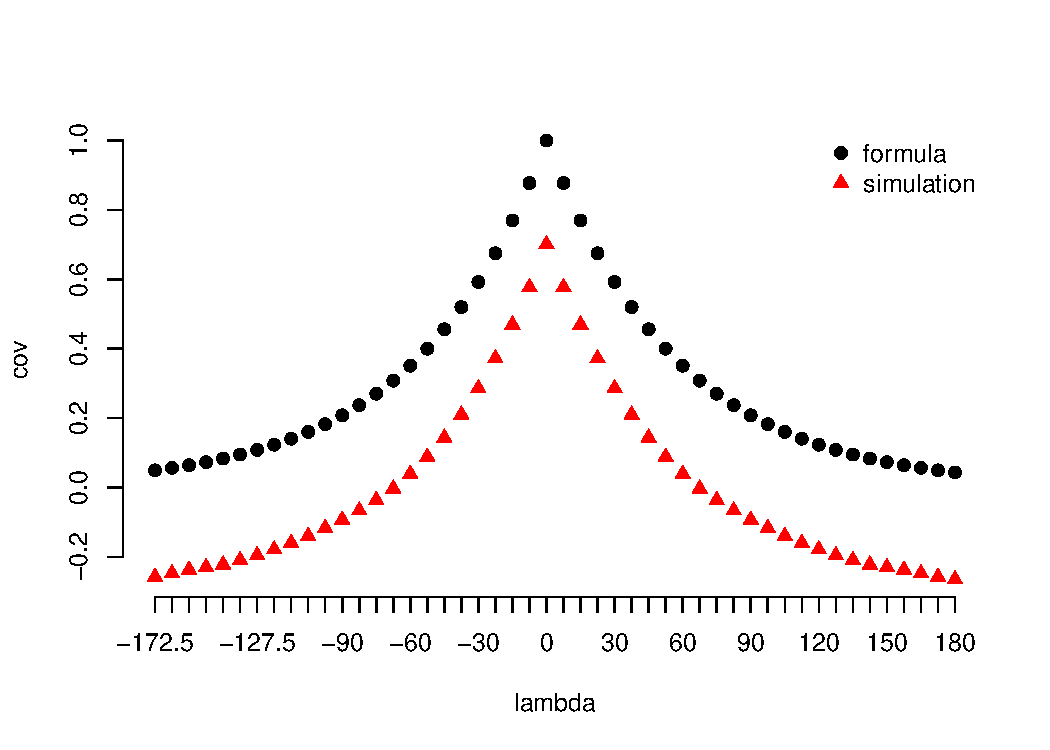
\includegraphics[width=0.65\textwidth]{graphs/Summary-covarince_circle_1}
%graph from data genaration summary doc line 177 
\caption {Theoretical and empirical covariance comparison comparison on a circle}
\end{figure}

covariance estimator without the mean term

\beq \label{cov:circle1}  
C(\theta) = \frac{1}{n_L} \sum_{i=1}^{n_L} (X(a_i+\theta) \cdot X(a_i)) 
\eeq

\begin{figure}
\centering
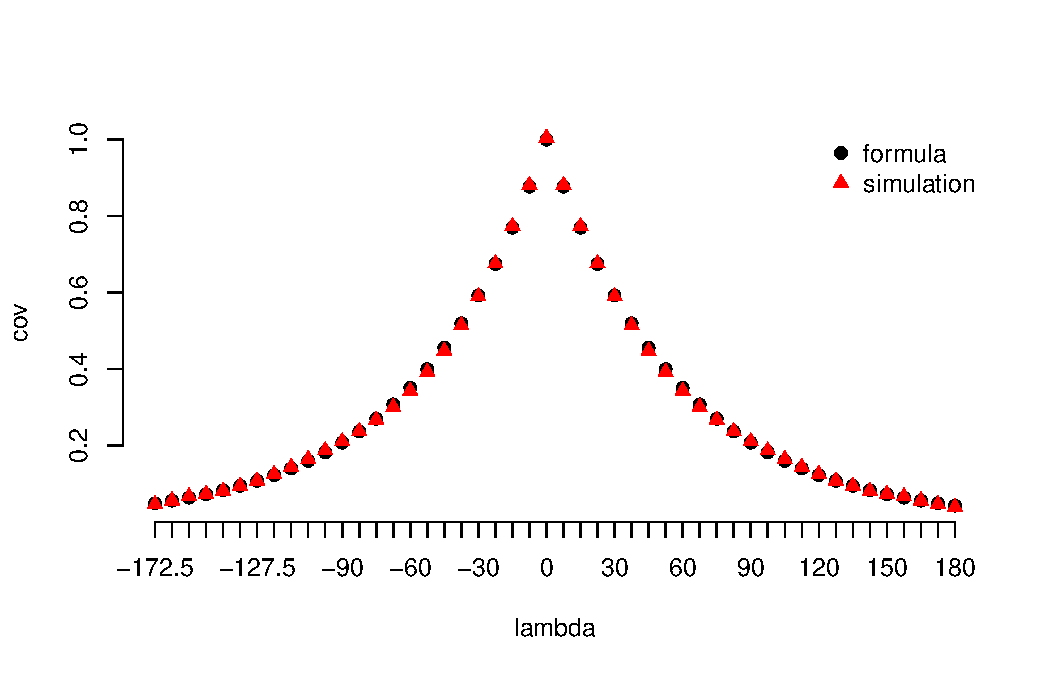
\includegraphics[width=0.65\textwidth]{graphs/Summary-covarince_circle_2}
%graph from data genaration summary doc line 194 
\caption {Theoretical and empirical covariance comparison comparison on a circle}
\end{figure}